\documentclass[a4paper]{article}
\newcommand{\sepspace}{\vspace*{1em}}	
%% Language and font encodings
\usepackage[english]{babel}
\usepackage[utf8x]{inputenc}
\usepackage[T1]{fontenc}
\usepackage{float}

%% Sets page size and margins
\usepackage[a4paper,top=3cm,bottom=2cm,left=3cm,right=3cm,marginparwidth=1.75cm]{geometry}

%% Useful packages
\usepackage{amsmath}
\usepackage{graphicx}
\usepackage[colorinlistoftodos]{todonotes}
\usepackage[colorlinks=true, allcolors=blue]{hyperref}

\title{ZND detonation of hydrogen and oxygen}
\author{Artur Abratanski}

\begin{document}
\maketitle


% pierwsza sekcja
\section{Introduction}\label{sec:intro}
In this report one will find a study about ZND detonation using mixture of oxygen and hydrogen. There is a connection between detonation cell size and induction time, which will be calculated in this paper. This program calculates induction time which usually is considered to equal zero.  
\section{Mathematical model}\label{sec:model}
ZND code has been downloaded from Caltech website, it's program calculating simple detonation, has been published for the first time in 1944. 

\section{Results}\label{sec:results}

\begin{figure}[H]
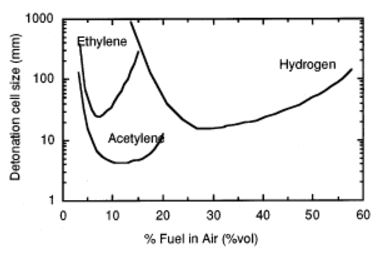
\includegraphics[width=1\textwidth]{cellsize.JPG}
\caption{\label{fig:cj}Experiments data}
\end{figure}

\begin{figure}[H]
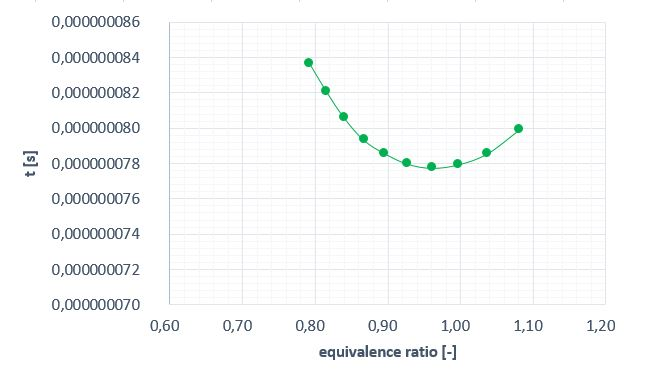
\includegraphics[width=1\textwidth]{ZND.JPG}
\caption{\label{fig:p}Calculated ZND detonation}
\end{figure}

These two charts has similar properties, there is a relation which will be calculated below:

\begin{equation}
    a = t_ind/\lambda=7,77E-08/0,0121=6,65E-06
 \end{equation}   

\section{Summary}\label{sec:summary}
Program for calculating ZND detonation produced related to experiments results. Induction time happened to be measured in $seconds^-8$. Detonation of hydrogen with oxygen is extremely fast, this is why this mixture is called Knallgas (Scandinavian and German Knallgas: "bang-gas").


\section{References}\label{sec:refs}

 
[1] ZND program  \newline
$http://shepherd.caltech.edu/EDL/public/cantera/html/SD_Toolbox/ZND$

[2] Properties of Hydrogen \newline
http://www.cnbyxf.com/Doc/data.WebNoteBooks2010/07/20100728122525



\end{document}
